% !TeX spellcheck = hu_HU
% !TeX encoding = UTF-8
\chapter{\bevezetes}

Az informatikában az adatbázis-kezelés területét az elmúlt közel 50 évben a relációs adatmodell dominálta. Mostanra azonban többen felismerték, hogy számos olyan alkalmazási terület van -- pl. közösségi hálók, ajánlórendszerek, pénzügyi csalások felderítése -- ahol az adatok gráf jellegű tárolása és feldolgozása előnyös lehet. A gráfadatbázisokban használt tulajdonsággráf (property graph) adatmodell hasznos eszköznek bizonyult sokféle probléma modellezésére, így az ezt használó eszközök az elmúlt évtizedben egyre népszerűbbek lettek, pl. a Neo4j gráfadatbázis-kezelő rendszer.\footnote{\url{https://neo4j.com/}} Az elmúlt években indult \mbox{openCypher} kezdeményezés célja pedig, hogy -- a relációs adatbázisokban alkalmazott SQL nyelv mintájára -- szabványos gráflekérdező nyelvet definiáljon.

\begin{figure}[!ht]
	\centering
	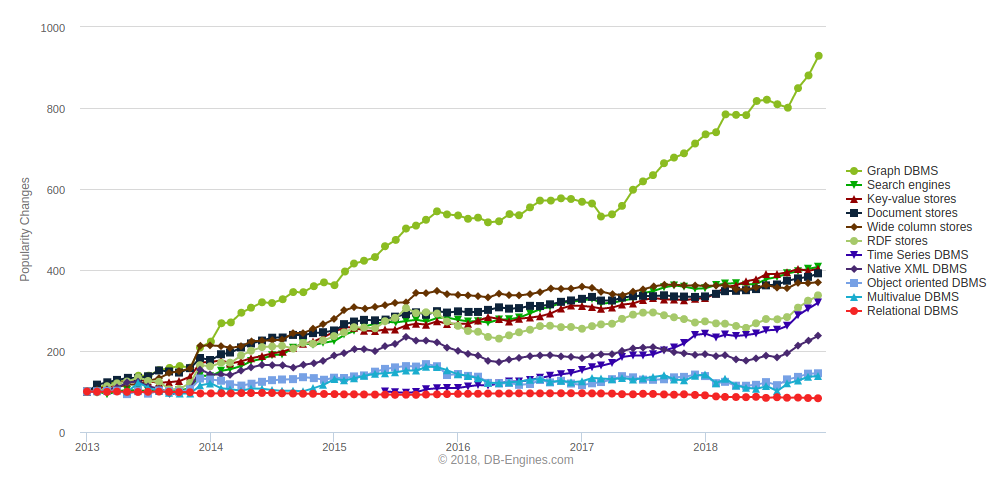
\includegraphics[width=150mm, keepaspectratio]{figures/graphdbms_trends.png}
	\caption{Adatbázisokban alkalmazott adatmodellek népszerűségének változása a \url{https://db-engines.com} oldal rangsorolása alapján}
	\label{fig:graphdbms_trends}
\end{figure}

Mi lehet a gráfadatbázisok \figref{graphdbms_trends}~ábrán is látható sikerének oka? Ezek a rendszerek több előnnyel is rendelkeznek a megszokott relációs adatbázisokhoz képest:

\begin{itemize}	
	\item \textbf{Intuitív adatmodell}: Az emberek szeretik úgy modellezni a világot, mint különböző entitások (csúcsok) és közöttük lévő kapcsolatok (élek) sokasága. Mind az entitások, mind a közöttük lévő kapcsolatok rendelkezhetnek különböző tulajdonságokkal, amelyek a tulajdonsággráfokkal egyszerűen kifejezhetőek.
	\item \textbf{Olvashatóság}: Ha megnézünk egy relációs adatbázison futtatott SQL  lekérdezést a séma ismerete nélkül, akkor nem magától értetődő, hogy egy attribútum egy tulajdonságot vagy kapcsolatot (idegen kulcs) jelent. A több-több kapcsolatoknál a kapcsolótáblák ezt egyértelműen meghatározzák, azonban a lekérdezés kevésbé olvasható lesz tőlük.
	\item \textbf{Tömörség}: Adott éltípusok mentén történő útkereső lekérdezéseket kifejezetten nehéz leírni SQL-ben és nem is minden SQL-dialektusban támogatottak. Még nehezebb a legrövidebb utat kereső lekérdezések megfogalmazása.
	\item \textbf{Gyors prototipizálás}: A gráfadatbázisok gyenge sémájának köszönhetően egyszerűbben létrehozhatók a prototípusok mint a relációs adatbázisoknál. Természetesen ennek következtében a lekérdezések optimalizálása bonyolultabbá válik a relációs lekérdezésekhez képest~\cite{DBLP:conf/cikm/SakrEH12}. Az egyik legnagyobb nehézséget a kapcsolatok kardinalitásának megbecslése jelenti körkörös illesztéseket tartalmazó lekérdezések esetében, melyre egy éltípuson történő ismételt navigálás megvalósításához van szükség. 
%	\item \textbf{Vizualizálás}: Egy gráfadatbázis, vagy annak részlete a megfelelő eszközök segítségével vizualizálva mélyebb betekintést adhat a teljes gráf struktúrájára vonatkozóan. Természetesen a megfelelő eszközök ritkák: a yWorks\footnote{\url{https://www.yworks.com/}} nevű cég yEd alkalmazása, vagy a Neo4j Bloom\footnote{\url{https://neo4j.com/bloom/}} alkalmazása nagyszerű, de használatuk nem ingyenes. A szabad szoftverek közül számos esetben egyedül a Graphviz\footnote{\url{https://www.graphviz.org/}} tud jó megjelenítést nyújtani.
\end{itemize}

A fentieket figyelembe véve elmondható, hogy sok esetben érthetőbb adathalmazt, valamint tömörebb lekérdezéseket eredményez a gráfadatbázisok használata. Azonban mivel ezek a rendszerek az informatika és a számítástudomány világában annyira újnak számítanak, hogy számos nyitott kérdés van velük kapcsolatban. Az egyik ilyen kérdés a gráfalapú lekérdezések és lekérdezőnyelvekkel kapcsolatos. Mivel a relációs adatbázisokban a -- legtöbbször SQL-ben megfogalmazott -- lekérdezések optimalizációjára igen hatékony megoldások léteznek, ezek bizonyos esetekben nem működnek jól a gráfadatbázisokban. Ezeknek az eseteknek az azonosítása az egyik legnagyobb nyitott kérdés. További fontos kérdés, hogy az ezeket a problémákat megoldó, illetve a már meglévő megoldások -- pl. a relációs adatbázisokban megszokott kétoperandusú illesztés (join) műveletek -- mennyire hatékonyak. Az alapvető problémák azonosításán és megoldásán túl fontos kérdés, hogy egyéb, a relációs adatbázisokban elterjed módszerek (pl. inkrementális nézetkarbantartás) hogyan ültethetőek át a gráfadatbázisokba.

Dolgozatomban megvizsgáltam, hogy mennyire hatékonyak a klasszikus relációs, és a modern gráfadatbázis-kezelők a gráfjellegű lekérdezések számítására.
Az ehhez szükséges elméleti háttér (\ref{sec:hatterismeretek}.~fejezet) megismerése után a kiértékeléshez kiválasztottam egy széleskörben elfogadott, sok nyelvi elemet és teljesítmény-aspektust lefedő teljesítménymérési keretrendszert, az LDBC Social Network Benchmarkot. A benchmark keretrendszerében javítottam a specifikáció hiányosságait és hibáit, ezek alapján frissítettem a benne található lekérdezéseket és szoftvermodulokat (\ref{sec:keretrendszer}.~fejezet).
A klasszikus adatbázis-kezelőkön kívül megvizsgáltam a differenciális adatfolyamot, mint alacsony válaszidővel rendelkező, elosztott, iteratív és inkrementális számításokat együttesen támogató számítási modellt. Az inkrementális lekérdezésekben nyújtott teljesítményének és a megközelítés használhatóságának tanulmányozásához a Transformation Tool Contest gráftranszformációs verseny (\ref{sec:ttc}.~fejezet) egyik feladatát valósítottam meg.
Az így rendelkezésre álló implementációk segítségével elkészítettem a különböző adatmodellt, nyelvet és megközelítést alkalmazó rendszerek összehasonlító teljesítménymérését (\ref{sec:kiertekeles}.~fejezet).
Végezetül áttekintettem a kapcsolódó kutatási eredményeket (\ref{sec:kapcsolodo}.~fejezet), amelyek alapján javaslatot tettem a tanszéken fejlesztett \emph{ingraph} rendszer továbbfejlesztésére. Végezetül pedig meghatároztam a további kutatási irányokat (\ref{sec:osszefoglalo}.~fejezet).
